\documentclass[a4paper]{article}

\usepackage{graphicx}
\usepackage{amsmath,amssymb}
\usepackage{minted}
\usepackage{multirow}
\usepackage{float}
\usepackage{todonotes}
\usepackage{forest}
\usepackage{xstring}
\usepackage{xcolor}
\usepackage[most]{tcolorbox}
\usepackage{xparse}
\usepackage{natbib}

\usetikzlibrary{graphs,graphdrawing}
\usegdlibrary{layered}

% for external graphviz
\input{/home/donkarlo/Dropbox/repo/nd_ai_project/src/nd_ai/knoweldge_representation/language/formal/computer/programming/tex/latex/code_clips/external_graphviz.tex}

% for tags
\input{/home/donkarlo/Dropbox/repo/nd_ai_project/src/nd_ai/knoweldge_representation/language/formal/computer/programming/tex/latex/parts/control_sequence/kind/semtag/semtag.tex}

% for links
\input{/home/donkarlo/Dropbox/repo/nd_ai_project/src/nd_ai/knoweldge_representation/language/formal/computer/programming/tex/latex/code_clips/seehere.tex}

\title{}
\date{}

\begin{document}
    \maketitle
    \cite{granley-2022-hybrid-neural-autoencoders} propose a topographic variational autoencoder to model proprioceptive neural coding in somatosensory cortex.
    The model is trained on natural human arm-movement kinematics, not directly on neural recordings, but reproduces several coding properties observed in monkey cortical neurons.
    The paper supports the idea that autoencoders can be used to model sensory representations and neural coding when the latent space is interpreted as a biologically constrained neural population.
    \begin{figure}[H]
        \centering
        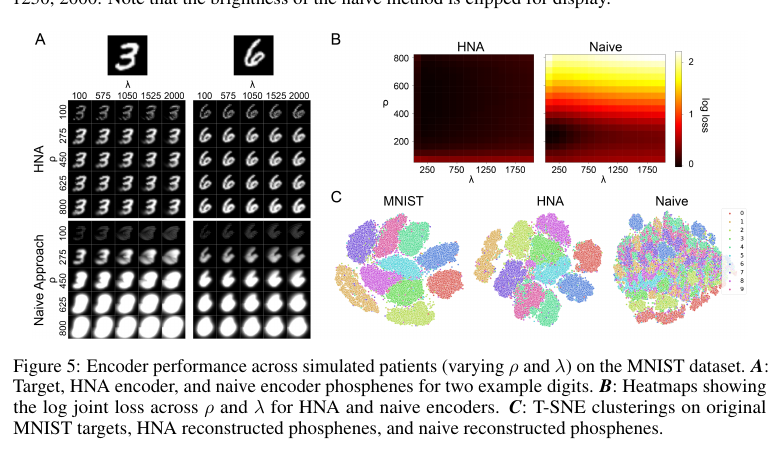
\includegraphics[width=0.9\textwidth]{granley-2022-hybrid-neural-autoencoders_figure_5.png}
    \end{figure}
    \bibliographystyle{plainnat}
    \bibliography{/home/donkarlo/Dropbox/repo/nd_shared_research/bibliography/bibliography.bib}
\end{document}